\documentclass[11pt]{article}
\usepackage[margin=1in]{geometry}
\usepackage{amsmath,amssymb,amsthm,bm,booktabs,microtype}
\usepackage[T1]{fontenc}
\usepackage{lmodern,xurl,graphicx}
\usepackage[colorlinks=true,allcolors=blue]{hyperref}
\hypersetup{pdftitle={Learning Spectral Geometry for Kernel Regression},pdfsubject={Single-bank spectral kernel regression and classification benchmarks},pdfauthor={Agus Sudjianto and Aijun Zhang},pdfkeywords={kernel ridge regression, spectral representation learning, metric learning, Laplace kernels, tabular learning, identifiable parameterization}}
\newcommand{\R}{\mathbb R}
\newcommand{\tr}{\operatorname{tr}}
\newcommand{\one}{\bm 1}
\newtheorem{proposition}{Proposition}
\title{Learning Spectral Geometry for Kernel Regression}
\author{Agus Sudjianto \and Aijun Zhang}
\date{October 2026}
\begin{document}
\maketitle
\begin{abstract}
We develop a learned spectral kernel for regression and classification on tabular data. The construction combines Fourier features with trainable frequencies, a positive-definite metric and a Laplace kernel. These components learn the scales of input variation, the directions relevant to prediction and the interactions induced by their joint distance. A canonical parameterization resolves amplitude--metric--bandwidth redundancy and gives a defined interpretation to feature and frequency weights. Supervised prediction loss trains the geometry, which then determines the kernel used in the final ridge fit. Experiments with numerical and categorical predictors show that a single spectral model is competitive with tuned gradient-boosted trees on several regression and classification tasks. Comparisons of approximate and exact ridge fits demonstrate that predictive accuracy depends jointly on the learned geometry and the quality of the regression fit. This separation of representation learning from task-specific prediction offers a framework for developing shared spectral representations through cross-task pretraining, toward tabular foundation models.
\end{abstract}
\noindent\textbf{Keywords:} Kernel ridge regression; spectral representation learning; metric learning; Laplace kernels; tabular learning; identifiable parameterization.
\par\medskip

\section{Introduction}
Gradient-boosted decision trees (GBDTs) are widely used for supervised learning on tabular data. XGBoost \cite{chen2016}, LightGBM \cite{ke2017} and CatBoost \cite{prokhorenkova2018} combine predictive performance with efficient implementations, including algorithms designed for large training sets. Their treatment of heterogeneous features and irregular response functions makes them relevant comparators for learned tabular representations. On a benchmark of medium-sized tables, with about 10,000 training samples, tree-based models outperformed the deep learning models evaluated by Grinsztajn et al.\ \cite{grinsztajn2022}.

Tabular foundation models introduce the possibility of reusing a learned representation across datasets. TabPFN, for example, is pretrained on synthetic tasks and predicts on a new table using its labeled examples as context \cite{hollmann2025}. Conventional boosted trees fit split thresholds and leaf values to a particular table and schema. Their partitions define a geometry for that task; transfer to tables with different columns requires additional structure.

Kernel regression provides such a separation. A learned kernel determines how observations are compared, while a regularized linear solve fits the coefficients of the predictor. The present paper develops and evaluates this construction within individual datasets. Cross-task learning would additionally require a representation that accommodates different feature schemas.

The choice of representation determines which differences between observations affect prediction. Standardized Euclidean distance assigns the same distance to a given input displacement throughout the feature space. In housing data, the predictive relevance of a change in income, occupancy or location can also depend on the other attributes of the observation. We therefore learn a nonlinear representation together with the metric used to compare its coordinates.

Fourier coordinates represent numerical variation at different scales. Each input is mapped to sine--cosine pairs whose frequencies are fitted to the prediction task: lower frequencies vary over longer input intervals and higher frequencies over shorter ones. This construction draws on the spectral representation of stationary kernels. Random Fourier features approximate a specified kernel \cite{rahimi2007}, while spectral mixture kernels learn a parametric spectrum \cite{wilson2013}. Here, the Fourier coordinates form a learned input representation. Finite frequency sets can map distant inputs to similar coordinates, so their behavior under extrapolation depends on the fitted frequencies.

A positive-definite metric weights directions in Fourier space and introduces cross terms between coordinates. These terms allow a joint change in location and income, for example, to contribute differently from either change considered separately. Feature masses and relative frequency amplitudes are recovered from the metric's diagonal blocks. Unequal stretching within a sine--cosine pair and coupling between pairs can make the resulting distance nonstationary in the original inputs.

The Laplace kernel converts this distance into similarity, with a learned bandwidth controlling its rate of decay. It preserves positive semidefiniteness after the learned transformation \cite[Theorem~1 and Corollary~1]{schoenberg1938}. Its exponent is linear in distance, giving a cusp at coincident observations, whereas the Gaussian kernel uses squared distance. Applying the Laplace function to a joint distance also gives a nonadditive similarity, including when the squared distance is a sum of featurewise contributions.

For the spectral map $u_\omega$, metric $B$ and bandwidth $T$, the kernel is
\begin{equation}
 k_\theta(x,x')=
 \exp\!\left[-\frac{\sqrt{(u_\omega(x)-u_\omega(x'))^\top
 B(u_\omega(x)-u_\omega(x'))}}{T}\right].
 \label{eq:intro-kernel}
\end{equation}
Kernel ridge regression uses~\eqref{eq:intro-kernel} in an expansion over training observations, with coefficients fitted jointly by a regularized solve. The construction belongs to the family of learned representations composed with kernels \cite{wilson2016}.

The same similarity admits a cross-attention interpretation. New observations supply queries, training observations supply keys and labels supply values. Row-normalized Laplace similarities yield a Nadaraya--Watson smoother in softmax form. Ridge regression uses the Gram matrix of pairwise training similarities to adjust the labels before aggregation. Section~\ref{sec:attention} derives both readouts; the experiments use ridge regression.

Learning amplitudes, a metric and a bandwidth independently introduces redundant scales. An amplitude change can be offset by the corresponding metric entries, and a uniform metric rescaling can be offset by the bandwidth. We impose unit trace on the metric and recover amplitudes and feature masses from its blocks. A symmetric trace-zero matrix exponential then gives unique coordinates for the positive-definite metric.

Each fitted model uses a single bank: one Fourier map, one metric and one bandwidth, followed by a ridge fit. On three matched California Housing splits, the refined model with exact ridge decoding has mean test root mean squared error (RMSE) of \$42,366, compared with \$43,186 for tuned CatBoost and \$43,568 for tuned LightGBM. Separate comparisons evaluate the decoder and geometry refinement. Experiments on hourly Bike Sharing, Taiwan credit default and Adult income extend the construction to mixed numerical and categorical inputs. 

\section{Spectral representation and kernel construction}
\subsection{Fourier representation}
For a continuous real stationary positive-semidefinite kernel with $k(0)=1$, Bochner's theorem gives a symmetric probability measure $\mu$ such that
\begin{equation}
 k(x-x')=\int_{\R^d}\cos\bigl(2\pi\xi^\top(x-x')\bigr)\,d\mu(\xi).
 \label{eq:bochner}
\end{equation}
Frequencies are measured in cycles per input unit, giving the factor $2\pi$. Rasmussen and Williams \cite[Theorem~4.1]{rasmussen2006} state the theorem in complex-exponential form; symmetry gives the real form in~\eqref{eq:bochner}.

Let $x\in\R^d$ denote an input after a fixed, training-fitted transformation. For feature $j$, $K$ positive ordered frequencies define
\begin{equation}
 u_{jk}(x)=\begin{bmatrix}\cos(2\pi\omega_{jk}x_j)\\ \sin(2\pi\omega_{jk}x_j)\end{bmatrix},
 \qquad u_\omega(x)=\operatorname{col}_{j,k}u_{jk}(x)\in\R^p,
 \qquad p=2dK.
 \label{eq:features}
\end{equation}
Each pair lies on the unit circle, and its angle changes by $2\pi\omega_{jk}$ per unit change in $x_j$. For pair weights $q_{jk}\geq0$, the identity
\begin{equation}
 \sum_{j,k}q_{jk}\|u_{jk}(x)-u_{jk}(x')\|^2
 =2\sum_{j,k}q_{jk}\{1-\cos[2\pi\omega_{jk}(x_j-x'_j)]\}
 \label{eq:chord}
\end{equation}
makes the induced stationary distance explicit. With weights summing to one, the corresponding weighted inner product is the atomic version of~\eqref{eq:bochner}.

Positive cumulative frequency gaps fix the sign and ordering conventions within each feature:
\begin{equation}
 \omega_{jk}=\sum_{\ell=1}^{k}\exp(\nu_{j\ell}),\qquad k=1,\ldots,K.
 \label{eq:gaps}
\end{equation}
Preprocessing fixes the input scale and coordinate origin; phase offsets are set to zero. These conventions address parameter redundancy; agreement of distinct frequencies on a finite sample is a separate source of observational equivalence.

\subsection{Metric shape and bandwidth}
For $\Delta u=u_\omega(x)-u_\omega(x')$, the metric distance and kernel are
\begin{equation}
 d_B(x,x')^2=\Delta u^\top B\Delta u,
 \qquad k_\theta(x,x')=\exp\{-d_B(x,x')/T\},
 \quad B\succeq0,\quad\tr B=1,\quad T>0.
 \label{eq:kernel}
\end{equation}
The eigenvectors of $B$ select directions in Fourier space; its eigenvalues determine their relative stretching. The bandwidth $T$ controls the overall distance scale.

The Euclidean Laplace kernel is positive semidefinite in any dimension \cite[Theorem~1 and Corollary~1]{schoenberg1938}, and composing it with a feature map preserves that property. Specifically, choose $R$ with $RR^\top=B$ and let $z(x)=R^\top u_\omega(x)$. Equation~\eqref{eq:kernel} is $\exp(-\|z(x)-z(x')\|/T)$, so every Gram matrix is positive semidefinite and $k_\theta(x,x)=1$.

Stationarity depends on the metric structure. Isotropic blocks for individual sine--cosine pairs, with zero cross blocks, recover the difference-only expression in~\eqref{eq:chord}. Unequal within-pair stretching and cross-pair terms can make the distance depend on the individual input locations. The frequencies characterize the representation, which can be used in both stationary and nonstationary kernels.

\section{Canonical parameterization}
Suppose a preliminary description has an amplitude matrix $D_0$, a metric $M$ and bandwidth $T_0$. Its squared scaled distance is
\begin{equation}
 \frac{\Delta u^\top D_0MD_0\Delta u}{T_0^2}
 =\Delta u^\top H\Delta u,
 \qquad H=\frac{D_0MD_0}{T_0^2}.
\end{equation}
Only $H$ enters the kernel, so independent amplitude, metric and bandwidth parameters admit equivalent descriptions of the same distance.

\begin{proposition}
For any nonzero positive-semidefinite $H$, the unique decomposition $H=B/T^2$ with $\tr B=1$ and $T>0$ is
\begin{equation}
 B=H/\tr H,\qquad T=(\tr H)^{-1/2}.
\end{equation}
\end{proposition}
\begin{proof}
Taking traces gives $\tr H=1/T^2$, which determines $T$ and then $B$.
\end{proof}

\subsection{Amplitude and feature weights}
Let $B_{jk,jk}$ be the $2\times2$ principal block for pair $(j,k)$. Define
\begin{equation}
 w_{jk}=\tr B_{jk,jk},\qquad
 \rho_j=\sum_k w_{jk},\qquad
 a_{jk}^2=\frac{w_{jk}}{\rho_j}.
 \label{eq:masses}
\end{equation}
Then $\sum_j\rho_j=1$ and $\sum_k a_{jk}^2=1$ whenever $\rho_j>0$. The feature mass $\rho_j$ records how much of the trace is assigned to feature $j$; $a_{jk}^2$ divides that mass among its frequencies. Both quantities are determined by the fitted $B$.

For positive pair masses, let $D$ have blocks $\sqrt{w_{jk}/2}\,I_2$. The remaining shape is
\begin{equation}
 \Gamma=D^{-1}BD^{-1},\qquad B=D\Gamma D,\qquad \tr \Gamma_{jk,jk}=2.
 \label{eq:shape}
\end{equation}
This is a unique decomposition under the stated block normalization. It separates allocation of mass from within-pair anisotropy and cross-pair coupling. If a pair mass is zero, this inverse is undefined; the zero-mass coordinates must be removed or treated as a boundary case. The positive-definite implementation below avoids that boundary.

Trace mass measures allocation within the representation. Predictive sensitivity also depends on frequency and cross terms, as derived below; correlated inputs further affect its interpretation.

\subsection{Matrix-exponential coordinates}
The positive-definite metric and bandwidth are parameterized by
\begin{equation}
 B(A)=\frac{\exp(A)}{\tr\exp(A)},\qquad A=A^\top,\quad\tr A=0,
 \qquad T=\exp(\tau).
 \label{eq:exponential}
\end{equation}
Matrix exponential methods for positive-definite trace-one matrices are established \cite{tsuda2005}. The restriction $\tr A=0$ removes the shift invariance $A\mapsto A+cI$.

\begin{proposition}
Equation~\eqref{eq:exponential} is a bijection between symmetric trace-zero matrices and positive-definite matrices of trace one. Its inverse is
\begin{equation}
 A=\log B-\frac{\tr(\log B)}p I.
 \label{eq:inverse}
\end{equation}
\end{proposition}
\begin{proof}
The exponential of a real symmetric matrix is positive definite. Normalizing its trace gives an admissible $B$. Conversely, the symmetric logarithm of a positive-definite $B$ exists uniquely. Subtracting its mean eigenvalue gives trace zero, and exponentiating recovers a positive scalar multiple of $B$. Trace normalization removes that scalar. Applying the same logarithm to any preimage gives~\eqref{eq:inverse}.
\end{proof}

Optimization uses $p(p+1)/2-1$ coefficients in an orthonormal basis of symmetric trace-zero matrices. Together with ordered frequencies and the block normalization, these coordinates fix frequency signs, permutations and compensating scales. Identifiability from observations also depends on the input sample: constant features, aliasing and equivalent representations can yield the same fitted kernel.

\section{Local sensitivity and feature interactions}
For a small displacement $h$,
\begin{equation}
 d_B(x,x+h)^2=h^\top J_u(x)^\top B J_u(x)h+o(\|h\|^2),
 \label{eq:local}
\end{equation}
where $J_u$ is the Fourier-map Jacobian. Thus $J_u(x)^\top B J_u(x)$ is the local metric in input coordinates. In the simple case $B_{jk,jk}=(w_{jk}/2)I_2$ with zero cross blocks, its $j$th diagonal entry is
\begin{equation}
 I_j=\frac12\sum_k w_{jk}(2\pi\omega_{jk})^2.
\end{equation}
Frequency and mass jointly determine sensitivity. A full $B$ adds cross-feature terms and allows sensitivity to vary with location.

The Laplace readout also makes the kernel nonadditive. Even if $d_B^2$ is a sum of featurewise distances, applying $\exp(-\sqrt{\cdot}/T)$ to that sum generally cannot be written as a sum of separate feature kernels. Consequently, a ridge expansion can express interactions. The bandwidth controls the decay of similarity with this joint distance.

The Euclidean Laplace kernel has a cusp at zero distance, whereas the squared-exponential kernel is smooth there. Their stationary spectra have different tails: under angular-frequency convention, the Laplace spectral density in $p$ dimensions is proportional to $(T^{-2}+\|\xi\|^2)^{-(p+1)/2}$, while the Gaussian spectrum decays exponentially in squared frequency \cite[Section~4.2.1, eq.~(4.15) with $\nu=1/2$]{rasmussen2006}.

\section{Geometry training and kernel regression}
\subsection{Support--query training}
Training episodes divide fitting observations into disjoint support and query sets $S,Q$. A kernel fit on $S$ predicts the labels in $Q$, and query error updates the geometry. For normalized targets $\widetilde y$ and support mean $\overline y_S$, the predictor and loss are
\begin{align}
 \widehat{\widetilde y}^{\rm ep}_q
 &=\overline y_S+k_{qS}(G_{SS}+\eta I)^{-1}
       (\widetilde y_S-\overline y_S\one),\\
 \mathcal L&=\frac1{|Q|}\sum_{q\in Q}
  (\widehat{\widetilde y}^{\rm ep}_q-\widetilde y_q)^2
       +\frac{10^{-4}}p\|A\|_F^2.
 \label{eq:episode}
\end{align}
Here $G_{SS}$ is the support Gram matrix, $k_{qS}$ contains the query-to-support kernel evaluations and $\eta>0$ is learned. Gradients pass through the support solve, Fourier map and matrix exponential. Both support and query observations are drawn from the designated fitting pool.

\subsection{Kernel ridge regression}
After geometry selection, the final fit minimizes squared error with an unpenalized intercept and a penalty in the reproducing kernel Hilbert space (RKHS) of $k_\theta$. For $\lambda>0$, the objective is
\begin{equation}
 \min_{b\in\R,\,f\in\mathcal H_{k_\theta}}
 \frac1n\sum_i(\widetilde y_i-b-f(x_i))^2+\lambda\|f\|_{\mathcal H_{k_\theta}}^2.
\end{equation}
The semiparametric representer theorem \cite[Theorem~2]{scholkopf2001}, with the constant function as the unpenalized component, gives a finite kernel expansion plus the intercept. For $G_{ij}=k_\theta(x_i,x_j)$ and $C_\lambda=G+n\lambda I$, its solution is
\begin{equation}
 b=\frac{\one^\top C_\lambda^{-1}\widetilde y}
          {\one^\top C_\lambda^{-1}\one},\qquad
 \alpha=C_\lambda^{-1}(\widetilde y-b\one),\qquad
 \one^\top\alpha=0.
 \label{eq:ridge}
\end{equation}
The two linear systems share a Cholesky factorization. With fitting-target mean $\mu_y$ and standard deviation $\sigma_y$, prediction in original units is
\begin{equation}
 \widehat y(x)=\mu_y+\sigma_y\left[b+\sum_i\alpha_i k_\theta(x,x_i)\right].
\end{equation}
The final intercept is estimated jointly with the kernel coefficients; episodic training centers the support labels by their sample mean. The regularizers follow the corresponding loss conventions: $\eta$ is the episodic diagonal shift and $n\lambda$ is the shift for the final mean-loss objective.

Nystr\"om approximation represents the kernel through a subset of training observations, called landmarks \cite{williams2001}. It reduces the cost of checkpoint selection and provides the approximate decoder in the experiments. Because the nonlinear Laplace readout can produce a full-rank Gram matrix from a compact embedding, the required landmark count must be assessed through the regression fit.

\begin{table}[htbp]
\centering\small
\caption{California Housing fitting protocol. The final ridge coefficients are fitted after geometry selection and outer-pool geometry refitting.}\label{tab:workflow}
\begin{tabular}{p{.21\linewidth}p{.70\linewidth}}\toprule
Stage & Operation\\\midrule
Preprocessing & Fit input and target transformations on the inner-training rows.\\
Geometry training & Draw disjoint support and query rows; compute Fourier coordinates and the normalized matrix exponential; differentiate query error through the support solve.\\
Validation & Select a geometry checkpoint, the final ridge penalty and optional output clipping using validation predictions.\\
Final fit & Freeze these choices, refit geometry for the selected number of steps on the outer-training pool, then fit the exact ridge head.\\
Prediction & Cache the selected metric transform and training embeddings; evaluate query similarities and apply the fitted coefficients.\\\bottomrule
\end{tabular}
\end{table}

\subsection{Relation to cross-attention}\label{sec:attention}
Scaled dot-product attention compares query representations with key representations from a context set and uses the resulting weights to combine the associated values \cite[Section~3.2.1]{vaswani2017}:
\begin{equation}
 \operatorname{Att}(\mathsf Q,\mathsf K,\mathsf V)
 =\operatorname{softmax}_{\rm row}
   \left(\frac{\mathsf Q\mathsf K^\top}{\sqrt{d_k}}\right)\mathsf V,
 \label{eq:standard-attention}
\end{equation}
where $d_k$ is the key dimension. In cross-attention the queries and the context come from different sets; here the queries are test observations $X_*$ and the context is the labeled training set $X$. The sans-serif matrices are representations, distinct from the episode sets $S,Q$ and the frequency count $K$.

The embedding $z(x)=B^{1/2}u_\omega(x)$ serves as both query and key representation. Define the distance score $\mathsf S$ and the cross-kernel matrix $G_{*X}$ by
\begin{equation}
 \mathsf S_{qi}=-\frac{\|z(x_q^*)-z(x_i)\|_2}{T},\qquad
 (G_{*X})_{qi}=e^{\mathsf S_{qi}}.
\end{equation}
Replacing the dot-product score in~\eqref{eq:standard-attention} with $\mathsf S$ and using the normalized labels as values gives
\begin{equation}
 W_{\rm att}=\operatorname{diag}(G_{*X}\one)^{-1}G_{*X}
             =\operatorname{softmax}_{\rm row}(\mathsf S),\qquad
 \widehat{\widetilde y}_*^{\rm NW}=W_{\rm att}\widetilde y.
 \label{eq:laplace-attention}
\end{equation}
This is the Nadaraya--Watson kernel smoother \cite{nadaraya1964,watson1964}, whose weights are positive and sum to one for each query.

The ridge predictor uses the same query--key similarities $G_{*X}$ but aggregates the fitted coefficients $\alpha$ of~\eqref{eq:ridge}, with no row normalization:
\begin{equation}
 \widehat{\widetilde y}_*^{\rm ridge}
 =b\one_*+G_{*X}\underbrace{(G+n\lambda I)^{-1}
                         (\widetilde y-b\one)}_{\alpha}.
 \label{eq:ridge-attention}
\end{equation}
The solve combines the labels using the training Gram matrix $G$, accounting for overlap among kernel functions centered on the training observations. Writing the predictor in terms of the labels makes the difference from~\eqref{eq:laplace-attention} explicit. For fixed geometry and $\lambda$, set
\begin{equation}
 c=C_\lambda^{-1}\one,\qquad s=\one^\top c,\qquad
 P=C_\lambda^{-1}-\frac{cc^\top}{s}.
\end{equation}
Substitution of~\eqref{eq:ridge} yields
\begin{equation}
 \widehat{\widetilde y}_*^{\rm ridge}=W_{\rm ridge}\widetilde y,
 \qquad W_{\rm ridge}=G_{*X}P+\frac{\one_*c^\top}{s},
 \qquad W_{\rm ridge}\one=\one_*,
 \label{eq:effective-ridge-weights}
\end{equation}
where the last identity follows from $P\one=0$. The unpenalized intercept makes the effective ridge weights sum to one, as the smoother's weights do, but individual ridge weights can be negative. These label weights differ from the expansion coefficients $\alpha$, which sum to zero. The identity holds for fixed geometry and before output clipping; because the geometry is itself learned from the labels, the full procedure is not linear in them.

\subsection{Categorical inputs and binary responses}\label{sec:mixed}
Categorical predictors require a representation independent of arbitrary numerical codes. For a categorical field with $c$ levels observed in the fitting pool, let $e_v\in\R^c$ be its indicator vector and let $\Phi\in\R^{c\times(c-1)}$ have orthonormal columns perpendicular to $\one$. The categorical coordinates are $\Phi^\top e_v$. This removes the constant direction of a full indicator encoding. A previously unseen level maps to zero, the centroid of the fitted level coordinates; a missing category is represented as an explicit level when present in training.

For mixed inputs, the representation concatenates the numerical Fourier pairs with these fixed categorical coordinates:
\begin{equation}
 u(x)=\operatorname{col}\bigl(u_\omega(x_{\rm num}),
                 \Phi_1^\top e_{v_1},\ldots,\Phi_m^\top e_{v_m}\bigr).
\end{equation}
Here $m$ is the number of categorical fields. One full trace-one metric acts on the concatenated representation, so the categorical fields can participate in cross terms with numerical features. The matrix-exponential parameterization and Laplace kernel are unchanged. Pair amplitudes in~\eqref{eq:masses} apply to the numerical Fourier blocks; a categorical field's trace mass is the trace of its corresponding principal block. Their block masses sum to the metric trace.

A binary target can be fitted with the same squared-error geometry objective and ridge head. For $y\in\{0,1\}$, the population squared-error minimizer is the conditional probability, although a fitted ridge score $s(x)$ need not lie in $[0,1]$. The classification experiments therefore use $s(x)$ for ranking and fit a sigmoid on a separate calibration set $\mathcal C$:
\begin{align}
 p(x)&=\{1+\exp[-(a s(x)+b_c)]\}^{-1},\\
 (\widehat a,\widehat b_c)
 &=\arg\min_{a,b_c}\sum_{i\in\mathcal C}
       \{-y_i\log p(x_i)-(1-y_i)\log[1-p(x_i)]\}
       +\frac{a^2}{2\mathcal R},\qquad \mathcal R=10^6.
\end{align}
The implementation uses logistic regression with an unpenalized intercept and weak slope regularization. Calibration rows are excluded from geometry training, ridge fitting and model selection. The same calibration procedure is applied to CatBoost's raw classification scores. Positive fitted slopes preserve score rankings; all reported calibration fits have positive slopes.

\section{California Housing experiment}
\subsection{Data and selection protocol}
California Housing contains 20,640 observations with eight numerical inputs; its source is the housing data studied by Pace and Barry \cite{pace1997}. We use the scikit-learn representation, with targets in units of \$100,000. For seeds $0,1,2$, random 80/20 splits yield 16,512 outer-training rows and 4,128 test rows. An inner 80/20 split, using random state $1000+s$, gives 13,209 fitting rows and 3,303 validation rows. Every comparator uses the same saved row indices. Input standardization and target mean and standard deviation are fitted only on the inner-fitting rows.

The selected spectral model has one bank, four frequencies per feature and $p=64$ coordinates. It has 2,079 metric coefficients, 32 frequency-gap coefficients and one log-bandwidth: 2,112 geometry parameters. Training adds one episodic diagonal-shift parameter, referred to as noise in the implementation.

The starting checkpoint comes from an earlier eight-configuration validation search. Each selected checkpoint used standardization, four frequencies initialized on a geometric grid between $0.025$ and $0.5$, and 300 training steps with 384 support and 256 query rows. Refinement starts from that saved checkpoint and uses 1,536 support and 512 query rows for up to 800 further steps. The recipe was chosen using seed zero's validation set and fixed for the remaining seeds. Appendix~\ref{app:training} gives optimizer details.

Checkpoints are compared every 200 steps using 2,048-landmark validation regression. For the selected checkpoint, an exact head chooses $\lambda$ from the nine-value grid $\{10^{-7+\ell/2}:\ell=0,\ldots,8\}$ and chooses whether to clip predictions to the fitting-label range. All three splits select step 800 and clipping. Their chosen $\lambda$ values are $10^{-6}$, $10^{-5.5}$ and $10^{-6}$.

After freezing those selections, each final run restarts from the same original checkpoint and performs the selected 800 refinement steps on all outer-training rows. The inner-fitted transformations are retained to preserve the warm-start coordinates. The exact head is then fitted on all outer-training rows. All three geometry checkpoints were saved before the new test evaluation. A separate ablation freezes the inner-refined geometry and refits only the head.

LightGBM \cite{ke2017} and CatBoost \cite{prokhorenkova2018} each receive a 16-configuration Sobol validation search, a 4,000-iteration cap and early stopping with patience 150. Each selected tree model is refitted on all outer-training rows for its selected iteration count. Search and computation budgets differ across methods. The California test splits had also been used in earlier exploratory work.

\subsection{Results}
Table~\ref{tab:results} reports mean and sample standard deviation across splits for RMSE and the coefficient of determination $R^2$. The refined model with full geometry refitting has mean RMSE \$820 below the retained tuned CatBoost baseline, a relative reduction of $1.90\%$. It has lower RMSE on each of the three matched splits (Table~\ref{tab:splits}).

\begin{table}[htbp]
\centering\small
\caption{California Housing test performance. All spectral rows use a single bank with four frequencies per feature. Standard deviations describe three overlapping random splits.}\label{tab:results}
\begin{tabular}{lrr}\toprule
Model & RMSE (dollars) & $R^2$ \\\midrule
Original spectral, Nystr\"om (2,048) & $46{,}517\pm1{,}380$ & $.8361\pm.0084$\\
Original spectral, exact head & $44{,}816\pm1{,}477$ & $.8479\pm.0088$\\
Refined spectral, frozen geometry & $42{,}444\pm1{,}112$ & $.8636\pm.0055$\\
Refined spectral, full refit & $\mathbf{42{,}366}\pm1{,}211$ & $\mathbf{.8641}\pm.0060$\\
Tuned LightGBM & $43{,}568\pm488$ & $.8563\pm.0026$\\
Tuned CatBoost & $43{,}186\pm932$ & $.8588\pm.0050$\\\bottomrule
\end{tabular}
\end{table}

\begin{table}[htbp]
\centering\small
\caption{Matched test RMSE in dollars. ``Frozen'' holds the inner-refined geometry fixed while fitting the exact head on all outer-training rows.}\label{tab:splits}
\begin{tabular}{rrrr}\toprule
Split seed & Spectral full refit & Spectral frozen & CatBoost\\\midrule
0 & 41,004 & 41,183 & 42,111\\
1 & 42,771 & 42,863 & 43,772\\
2 & 43,323 & 43,286 & 43,674\\\bottomrule
\end{tabular}
\end{table}

Replacing the initial approximate decoder with an exact head reduces mean RMSE by about \$1,700 without changing that geometry. The exact head reselects its regularizer and clipping on validation, so this difference reflects the full decoder change, including that reselection. Further geometry refinement reduces error by roughly another \$2,372 with geometry held fixed during the outer refit. That refinement changes support size, learning rates and optimization budget together. Refining geometry on the full outer-training pool provides a smaller additional mean reduction of about \$78. On split seed 2, the frozen geometry has RMSE \$43,286 against \$43,323 for the full refit (Table~\ref{tab:splits}).

The full-refit margins over CatBoost on the three splits are \$1,107, \$1,001 and \$351. The three overlapping splits provide limited evidence about performance differences across independent samples. Results on other datasets are reported in Section~\ref{sec:extended}.

\subsection{Learned spectral geometry}
Figure~\ref{fig:geometry} shows the full-refit model for split zero. The metric assigns approximately $44.96\%$ of its trace to latitude and $31.48\%$ to longitude, a combined $76.44\%$. Local sensitivity also depends on frequencies and cross terms through~\eqref{eq:local}.

\begin{figure}[htbp]
\centering
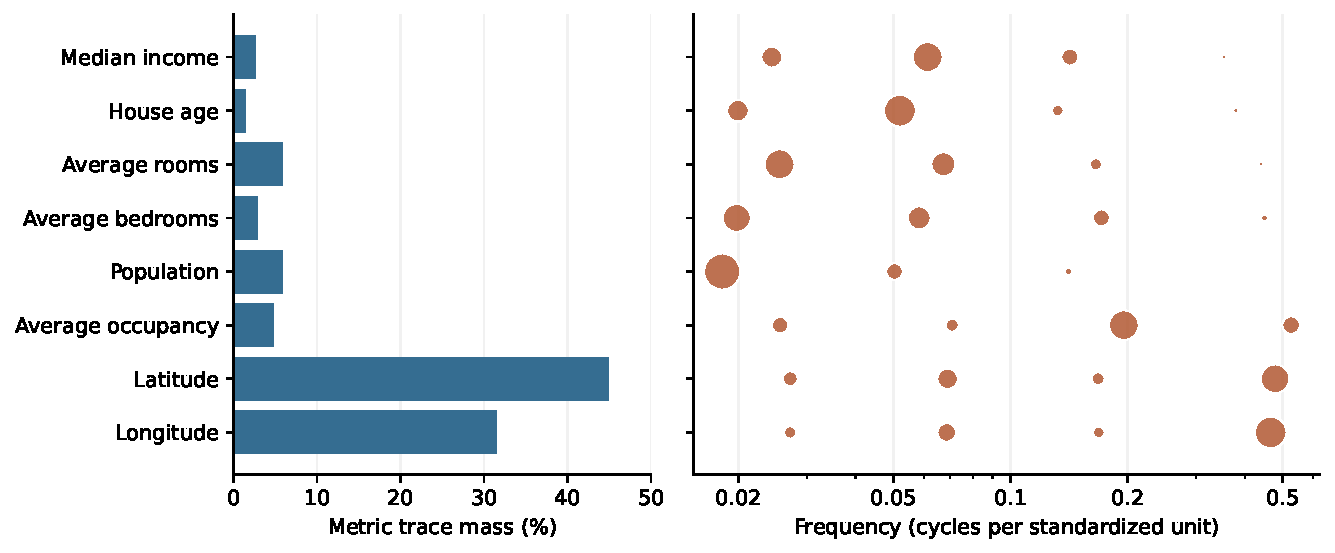
\includegraphics[width=\linewidth]{identifiable_spectral_geometry.pdf}
\caption{Saved single-bank geometry for split zero after the full refit. Left: each feature's metric trace mass $\rho_j$. Right: its four learned frequencies in cycles per standardized input unit; marker area is proportional to the within-feature mass $a_{jk}^2$. The panels are computed from saved checkpoint diagnostics.}\label{fig:geometry}
\end{figure}

\subsection{Computation and numerical checks}
The symmetric matrix exponential is evaluated through
\begin{equation}
 R(A)=\frac{\exp(A/2)}{\|\exp(A/2)\|_F},\qquad RR^\top=B(A),
 \qquad z(x)=R(A)^\top u_\omega(x).
 \label{eq:root}
\end{equation}
This identity evaluates the full metric through its symmetric square root. Appendix~\ref{app:derivative} gives the matrix-exponential derivative.

A dense matrix exponential costs $O(p^3)$ arithmetic. Transforming $n$ embeddings costs $O(np^2)$; forming all pairwise distances costs $O(n^2p)$. Exact ridge factorization costs $O(n^3)$ and requires $O(n^2)$ storage. Representation dimension governs the exponential cost, while support size governs the kernel matrix and ridge factorization. At $n=16{,}512$, one float64 Gram matrix occupies about 2.18 GB (2.03 GiB), before factors, cross-kernels and workspace.

Once the geometry is frozen, $R(A)$ and the training embeddings can be cached. Prediction then requires Fourier evaluation, the fixed linear transform and kernel evaluations, with no new matrix exponential. During training, changing $A$ requires updating the exponential and differentiating through it. The timings below aggregate these operations within each training or fitting stage.

On the NVIDIA GB10 GPU in float64, mean additional geometry-selection time was 165.9 seconds per split, full geometry refitting took 136.0 seconds, and exact final head fitting plus prediction took 8.9 seconds. These timings cover the selected refinement and final fit; the initialization search and exploratory candidates are additional costs.

The saved audit recomputes metrics from predictions, checks identical split indices, verifies the canonical constraints and inverse and checks relative exact-solve residuals below $10^{-9}$. Source snapshots, selection records and predictions accompany the results.

\section{Additional regression and classification experiments}\label{sec:extended}

Hourly Bike Sharing, Taiwan credit default and Adult income test the same single-bank construction beyond California Housing \cite{fanaee2013data,yeh2009data,becker1996data}. The mixed-input representation and binary-response readout are specified in Section~\ref{sec:mixed}. These runs train geometry from scratch; they do not reuse the California geometry.

\subsection{Data and evaluation protocol}

The hourly Bike Sharing file contains 17,379 observations. Its \texttt{casual} and \texttt{registered} columns sum to the target and are excluded, together with the row identifier and date string. The retained predictors describe calendar time and observed weather. The first 60\% of dates provide 10,389 fitting rows, the next 20\% provide 3,502 validation rows and the final dates provide 3,488 test rows. Training ends on March 13, 2012, and testing begins on August 7, 2012. Three optimizer seeds use this same chronology. The task predicts counts from observed covariates; it does not evaluate forecasting with unavailable future weather.

Taiwan contains 30,000 observations with 23 predictors and a binary next-month default label. Three stratified splits each allocate 19,200 rows to fitting, 2,400 to calibration, 2,400 to validation and 6,000 to testing. The numerical amounts retain their original values. Sex, education and marital status are treated as categorical fields.

Adult predicts whether annual income exceeds \$50,000 from 14 census attributes. The official 16,281-row test partition is retained. For each of three seeds, the original 32,561 training rows are divided into 26,048 fitting, 3,256 calibration and 3,257 validation rows. Missing categories are represented explicitly and all rows are retained. The sampling-weight attribute is used as an input feature; the reported metrics are unweighted.

Both model families use identical row assignments. Calibration and validation observations remain outside the final model fit; these added experiments do not perform the outer-pool refit used for California. ROC AUC, the area under the receiver operating characteristic curve, selects classification models. A separate sigmoid fit on calibration observations supplies probabilities for log loss, Brier score and accuracy. RMSE selects regression models.

\subsection{Training and selection}

The spectral representation has four frequencies per numerical feature. Fixed categorical contrasts are appended before applying the full metric. Numerical standardization and a quantile-to-normal transformation are compared on seed zero. Its selected preprocessing recipe is then fixed for seeds one and two. Each model trains for up to 800 steps using 1,024 support rows and 256 disjoint query rows. Checkpoints at steps 0, 200, 400, 600 and 800 are compared with a 512-landmark head. The selected checkpoint is evaluated with 2,048 landmarks over the nine-value ridge grid used for California. Exact validation solves compare the resulting ridge and its adjacent grid values. This limits the number of dense factorizations and does not exhaust the exact-head search space.

Adam begins at learning rate 0.01 for diagonal metric coordinates, log bandwidth and log noise, and 0.002 for off-diagonal coordinates and log-frequency gaps. Rates decay to 20\% of these values by the cosine schedule. The episode penalty, parameter bounds and gradient clipping follow the earlier construction. Target standardization is fitted on fitting rows and is also used for binary-label squared-error training.

CatBoost receives 16 Sobol configurations on seed zero, at most 3,000 trees per configuration and early stopping with patience 150. The selected configuration is fixed for the other two seeds, which retain their own stopping iterations. CatBoost uses native categorical processing. Every spectral and CatBoost selection is saved before any test prediction; the search budgets differ between families.

\subsection{Results}

\begin{table}[htbp]\centering\small

\caption{Hourly Bike Sharing test results on the fixed chronological holdout. Standard deviations describe three training runs on the same test rows.}\label{tab:bike}

\begin{tabular}{lrrr}\toprule Model & RMSE & MAE & $R^2$\\\midrule

Spectral kernel & $92.61\pm1.25$ & $64.23\pm0.88$ & $0.8236\pm0.0047$\\

Tuned CatBoost & $107.45\pm6.87$ & $75.78\pm5.91$ & $0.7619\pm0.0298$\\

\bottomrule\end{tabular}\end{table}

\begin{table}[htbp]\centering\small

\caption{Binary classification test results after separate sigmoid calibration. Larger AUC and smaller log loss or Brier score indicate better performance. Adult runs share the official test partition.}\label{tab:classification}

\begin{tabular}{llrrrr}\toprule Dataset & Model & AUC & Log loss & Brier & Accuracy\\\midrule

Taiwan & Spectral & $0.7873\pm0.0021$ & $0.4277\pm0.0024$ & $0.1339\pm0.0009$ & $0.8213\pm0.0025$\\

Taiwan & CatBoost & $0.7828\pm0.0027$ & $0.4276\pm0.0014$ & $0.1340\pm0.0005$ & $0.8213\pm0.0013$\\

Adult & Spectral & $0.9147\pm0.0005$ & $0.3153\pm0.0017$ & $0.0983\pm0.0006$ & $0.8620\pm0.0008$\\

Adult & CatBoost & $0.9274\pm0.0005$ & $0.2775\pm0.0008$ & $0.0880\pm0.0002$ & $0.8736\pm0.0007$\\

\bottomrule\end{tabular}\end{table}

Tables~\ref{tab:bike} and~\ref{tab:classification} report every added dataset under the frozen protocol. Variation across the three Bike Sharing runs reflects training randomness on one chronology. Adult varies the fitting and calibration partitions while retaining one official test set. Those standard deviations do not estimate uncertainty across independent test samples. Component ablations and comparisons under matched computational budgets remain outside this experiment.

The independent audit verifies all 18 model runs, including source-file hashes, split identity, validation selections, calibration separation, positive metric eigenvalues, ridge residuals and prediction replay. The accompanying source, per-run records and audits are listed in Appendix~\ref{app:repro}.


\section{Discussion}
The fitted geometry can be examined through its frequencies, trace allocation and cross terms. Their effects depend on one another: local sensitivity depends jointly on frequency and metric weight, as shown in~\eqref{eq:local}. The canonical parameterization fixes the scale conventions needed to compare these quantities across fitted models.

With geometry held fixed, the exact ridge fit reduces prediction error relative to the landmark approximation. A scalable implementation must therefore control approximation error in the regression fit as well as in the representation. The matrix exponential and ridge factorization require separate computational strategies because they depend on representation dimension and training size, respectively.

The California comparison reflects exploratory development on reused holdouts. The additional datasets follow the fixed protocol of Section~\ref{sec:extended}, with different tuning budgets for the spectral and tree models. Further evaluation should include matched budgets, geographic blocking for California and comparisons with fixed frequencies, diagonal metrics and Gaussian kernels to isolate the contribution of each component.

The added datasets distinguish ranking from probability quality. On Taiwan, the spectral AUC exceeds CatBoost's by 0.003 to 0.006 on each split, while the calibrated log losses agree to within 0.0011. The Bike Sharing comparison rests on one time boundary with observed weather.

On Adult the single-bank model has lower predictive performance than CatBoost: its mean test AUC is 0.9147 against 0.9274, and its calibrated log loss is 0.3153 against 0.2775. Each reported fit uses one spectral map, one metric and one bandwidth across its training population. Whether the Adult gap comes from this shared geometry, preprocessing, the training objective or incomplete optimization remains open.

\section{Conclusion}
The learned spectral kernel expresses tabular prediction through a fitted geometry and a regularized regression model. Ordered Fourier frequencies describe variation at different scales, while the metric determines how those coordinates contribute jointly to distance. Canonical normalization gives feature and frequency weights a defined scale and separates them from the bandwidth.

The single-bank model is competitive with tuned boosted trees on several tasks, while CatBoost predicts Adult income more accurately. The decoder comparisons show that geometry learning and the final ridge fit must be considered together: improving the regression approximation changes predictive accuracy even with the representation held fixed. Scalable readouts should be evaluated against the prediction quality of the exact fit.

Cross-task pretraining is a further direction for tabular foundation modeling. It requires a shared representation for tables with different schemas and a training objective spanning tasks. The spectral construction provides a model in which those representations, their induced geometry and the task-specific regression fit can be studied separately. Evaluation on unseen tables would determine how much of that geometry transfers and how much fitting a new task requires.

\appendix
\section{Optimizer coordinates and refinement settings}\label{app:training}
The diagonal basis consists of $p-1$ Helmert vectors $h_r$, $r=1,\ldots,p-1$: the first $r$ entries equal $1/\sqrt{r(r+1)}$, entry $r+1$ equals $-r/\sqrt{r(r+1)}$, and the rest are zero. Together with symmetric off-diagonal basis elements,
\begin{equation}
 A=\sum_{r=1}^{p-1}\beta_r\operatorname{diag}(h_r)
   +\sum_{a<b}\gamma_{ab}\frac{e_ae_b^\top+e_be_a^\top}{\sqrt2}.
\end{equation}
This basis is orthonormal under the Frobenius inner product and has no free trace direction. For $p=64$, it contains $63+2{,}016=2{,}079$ coefficients.

The initial search combines standard or quantile preprocessing, $K\in\{4,8\}$, and two paired settings of learning rate and initial maximum frequency: $(0.02,0.5)$ and $(0.04,1.5)$. All three selected initial models use standardization, $K=4$, and the first pair. Initial validation uses 512 landmarks; a subsequent rank selection compares 512, 1,024 and 2,048, selecting 2,048 on every split.

Refinement uses Adam with initial learning rate $0.003$ for diagonal metric coefficients, $\tau$ and log-noise, and $0.0006$ for off-diagonal coefficients and frequency gaps. At step $t$, both rates are multiplied by $0.2+0.4[1+\cos(\pi t/800)]$. The gradient norm is clipped at 10. Log-gaps are bounded to $[-9,2]$, $\tau$ to $[-5,3]$, and noise to $[10^{-4},1]$, initialized at $0.1$. If the eigenvalue spread of $A$ exceeds 20, its coordinates are uniformly rescaled to spread 20. Since $\kappa(B)=\exp(\lambda_{\max}(A)-\lambda_{\min}(A))$, this bounds the metric condition number by $e^{20}$. Checkpoint validation uses the same nine-value ridge grid as exact-head selection.

\section{Matrix-exponential differentiation}\label{app:derivative}
For a symmetric perturbation $E$, define the Fr\'echet derivative
\begin{equation}
 L_A[E]=\left.\frac{d}{dt}\exp(A+tE)\right|_{t=0}
       =\int_0^1\exp((1-s)A)E\exp(sA)\,ds.
\end{equation}
Numerical methods for this derivative are studied by Al-Mohy and Higham \cite{almohy2009}. Applying the quotient rule to~\eqref{eq:exponential} gives
\begin{equation}
 DB(A)[E]=\frac{L_A[E]-B(A)\tr L_A[E]}{\tr\exp(A)}.
\end{equation}
Its trace is zero, as required for a perturbation along the unit-trace surface. If $A=V\operatorname{diag}(a)V^\top$, the equivalent expression is
\begin{equation}
 L_A[E]=V\bigl(F\odot(V^\top EV)\bigr)V^\top,\qquad
 F_{rs}=\begin{cases}
 (e^{a_r}-e^{a_s})/(a_r-a_s),&a_r\ne a_s,\\
 e^{a_r},&a_r=a_s.
 \end{cases}
\end{equation}
The repeated-eigenvalue case uses the continuous divided-difference limit. The implementation differentiates the dense matrix exponential through automatic differentiation.

\section{Code and reproducibility}\label{app:repro}
The implementation, recorded checkpoints, prediction arrays and manuscript are available at \url{https://github.com/asudjianto-xml/Tabular-Spectral-Kernel}. Release \texttt{v0.1.0} contains the single-bank experiments reported here. Installation instructions and the distinction between verification, replay and training are given in \path{README.md} and \path{REPRODUCIBILITY.md}.

The package accepts data and output directories from the command line. Public datasets are downloaded into the specified cache. A small synthetic CPU run checks differentiation through the matrix exponential and ridge solve. For example:
\begin{verbatim}
tsk smoke --device cpu --output runs/install-check
tsk verify --output runs/recorded-audit
tsk download --dataset all --data-dir data
tsk reproduce --dataset bike --mode replay --seeds 0 \
  --device auto --data-dir data --output runs/bike-replay
\end{verbatim}

Verification recomputes per-run metrics from the bundled predictions, checks split separation and artifact hashes and exports aggregated results as a CSV file. The \texttt{assets} command regenerates the learned-geometry figure. Replay loads the recorded geometry and rebuilds its exact ridge head from the public data, comparing predictions with the saved arrays. Training repeats the documented fitting protocol and can produce different results across numerical platforms.

Source files are under \path{src/tabular_spectral_kernel/}, with the experiment implementations in \path{_paper/} and the saved evidence in \path{recorded/}. California training uses the published inner-training warm starts by default. The initialization search can also be rerun. The release retains the selected single-bank refinement recipe from the historical adaptive screen. The additional-task commands repeat preprocessing selection, geometry fitting, ridge selection, tree tuning and calibration before test evaluation.

The recorded environment uses PyTorch 2.13.0+cu130, NumPy 1.26.4, scikit-learn 1.6.1, CatBoost 1.2.10 and LightGBM 4.7.0. The repository records these versions separately from the supported installation dependencies. CPU execution is available, but the dense exact heads still require quadratic memory and cubic factorization work. Reference metadata and the claims checked against primary sources are recorded in \path{paper/identifiable_spectral_reference_audit.json}.

\bibliographystyle{plain}
\bibliography{identifiable_spectral_regression}
\end{document}
